\documentclass[a4paper,10pt]{article}
\usepackage{graphicx}
\usepackage{verbatim}
\usepackage{subfig}
\usepackage{float}
\usepackage[spanish]{babel}   %ver bien como es
\usepackage[utf8]{inputenc}
\usepackage{tabularx}
\hyphenation{des-com-po-ner-los va-rie-dad in-gre-dien-tes ac-tua-li-za-cio-nes me-dian-te con-si-de-ra-cio-nes nues-tro au-to-ma-ti-za-do pro-pues-tos con-tras-ta-das ra-zo-na-ble}

\begin{document}

\tableofcontents

\newpage


\section*{Introducci\'on}
\addcontentsline{toc}{section}{Introducci\'on}


\newpage
\section*{Presunciones}
\addcontentsline{toc}{section}{Presunciones}


\newpage


\section*{Vistas}
\addcontentsline{toc}{section}{Vistas}
En esta secci\'on presentaremos las diferentes especificaciones realizadas durante el presenta trabajo pr\'actico.
Se explicar\'a como se abord\'o cada parte del trabajo, explicando para que momentos fue utilizada cada t\'ecnica de especificaci\'on, y el porque
de esta desici\'on.

En un aspecto general, se divieron las t\'ecnicas de especificaci\'on seg\'un los siguientes crit\'erios:

\begin{itemize}
\item Modelo Conceptual: Se utilizar\'a para un entendimiento global del funcionamiento del sofware, entiendendo las entidades que interactuan dentro y con el mismo.
\item Diagrama de Casos de Uso: Se utilizar\'a para mostrar todas las interacciones que la m\'aquina tiene con los diversos actores.
\item Diagramas de Actividad: Se utilizar\'an para mostrar secuencias de acciones, usualmente agruparan diversos casos de uso que posean un hilo conductor.
\item Maquinas de Estado Finitas: Se utilizar\'an para mostrar las acciones que ocurren principalmente dentro de la m\'aquina para de esta manera, junto a los dem\'as esqumas
, poder dar un panorama completo del comportamiento del software.
\end{itemize}


\bigskip

\subsection*{Modelo Conceptual}
\addcontentsline{toc}{subsection}{Modelo Conceptual}

El modelo conceptual es una primera aproximaci\'on a todo lo que se quiere describir detalladamente en el transcurso de este trabajo. Explica 
de manera temprana la relaci\'on que existe entre los actores externos y las diferentes partes que componen a la pizzer\'ia para lograr un buen
entendimiento de las interconexiones presentes sin indicar ning\'un tipo de comportamiento por el momento.

A continuaci\'on se presenta el diagrama realizado para este modelo, seguido de las pertinentes explicaciones.

% Aca va el diagrama del modelo conceptual


\medskip

Del diagrama anterior se explayan los siguientes puntos para un mejor entendimiento:

\begin{itemize}
\item Dado que hay diferentes cargos dentro del personal se decidi\'o por utilizar el recurso de herencia para identificarlos. Si bien cada subclase
no tiene ning\'un atributo muy distintivo, el repositor tiene algunas relaciones particulares. Este fue el factor determinante para elegir usar herencia
y no poner el tipo de personal como un atributo enumerado, ya que entonces habr\'ia que poner las relaciones del repositor a personal y luego 
restringir por OCL que el relacionado sea de tipo repositor.
\item Por la clase men\'u se entiende el men\'u que la pizzer\'ia ofrece m\'as all\'a del stock que se encuentre disponible.
\item Por la clase producto se entiende cualquier producto que la pizzer\'ia alguna vez ofreci\'o. Esto se realiz\'o de esta manera dado que pensar 
los productos solamente como los que se encuentran en el men\'u podr\'ia traer inconsistencias. Un cliente puede realizar un pedido que contenga un producto
que est\'a en el men\'u (y haya stock para realizarlo), pero una vez hecho este pedido, el producto podr\'ia ser removido del men\'u en una actualizaci\'on,
y a\'un as\'i el pedido con el producto desaparecido del men\'u podr\'ia perdurar en el sistema dado que no se realiz\'o todav\'ia. Es por esto que
pueden existir productos por fuera del men\'u.
\item El cliente esta pensado como una persona o un grupo de personas dentro un local, por eso la multiplicidad cliente-local es uno. Si esa persona
o grupo de personas se movilizacen hac\'ia otro local no hay raz\'on para no pensarlos como un nuevo cliente dentro del otro local.
\item Un pedido de reposici\'on esta conformado por ingrendientes y sus cantidades pedidas, por lo que se opt\'o por utilizar una agregaci\'on calificada
para modelar esto.
\end{itemize}

Cosas que no me gustan aca:

habria que cambiar la relacion de pedidorepo-repositor, por pedidorepo-impresora
el mozo por ahi deberia estar unido a cliente
ver en general toda la validez del modelo


\medskip

A continuaci\'on se detallar\'an las restricciones sobre el modelo que no se desprenden del diagrama mediante el lenguaje OCL, indicando en cada
caso que fue lo que se quizo restringir en idioma castellano.

\medskip


Se explicitaron las correspondencias de cada local con cada tipo de empleado (clase personal y sus subclases).


\underline{context Local}

self.personal$\rightarrow$select(p$|$p.isKindOf(Jefe de Chefs)).size()$=1$

self.personal$\rightarrow$select(p$|$p.isKindOf(Cocinero)).size()$>0$

self.personal$\rightarrow$select(p$|$p.isKindOf(Mozo)).size()$>0$

self.personal$\rightarrow$select(p$|$p.isKindOf(Operador)).size()$=1$

self.personal$\rightarrow$select(p$|$p.isKindOf(Repositor)).size()$=1$

\medskip

El men\'u es el mismo para todos los locales.

\underline{context Local}

Local.allInstances().men\'u$\rightarrow$asSet()$\rightarrow$size()$=1$

\medskip

Para todo dep\'osito, cada ingrediente cuyo nivel de stock se encuentre por debajo de mínimo tolerable tiene que estar en un \'unico pedido de reposición relacionado con el local correspondiente al dep\'osito en cuesti\'on.

\underline{context Depósito de stock}

self.ingrediente$\rightarrow$select(i|i.disponibilidad.cantidad$<$disponibilidad.límite)$\rightarrow$

forAll(i$|$i.pedidodereposición.size()$=1$ and i.pedidodereposición$\rightarrow$forAll(p$|$p.local.depósitodestock$=$self))

\medskip

Explicar mejor
Se pide, para un pedido de reposici\'on, una cantidad de stock mayor o igual al límite tolerable de los ingredientes que se encuentran en el pedido de reposición. 
Esto es as\'i para que una vez que se realiza el pedido, seguro se cuente con el m\'inimo necesario.

\underline{context Ingredientes}

self.pedidodereposición$\rightarrow$.forAll(p|p.cantidad$\geq$self.disponibilidad.límite)


\medskip

La impresora utilizada en un pedido de reposición es la impresora del local que emitió dicho pedido.

\underline{context Pedido de reposición}

self.Impresora$=$self.Local.Impresora


\newpage

\subsection*{Diagrama de Casos de Uso}
\addcontentsline{toc}{subsection}{Diagrama de Casos de Uso}

Esta t\'ecnica sirve para mostrar como son las interacciones entre el mundo y la m\'aquina, es decir que se abstraen varias de las relaciones presentes
obviando las relaciones prop\'ias entre actores que se encuentran por fuera de la m\'aquina, as\'i como las interacciones que son intr\'insecas de la m\'aquina.

\subsubsection*{Diagrama}
\addcontentsline{toc}{subsubsection}{Diagrama}

A continuaci\'on se presenta el diagrama de casos de uso para toda la m\'aquina, es decir, se engloban todas las interacciones en un mismo diagrama
y luego se detallar\'a en particular cada caso de uso.


\begin{figure}[H]
\centering
\subfloat{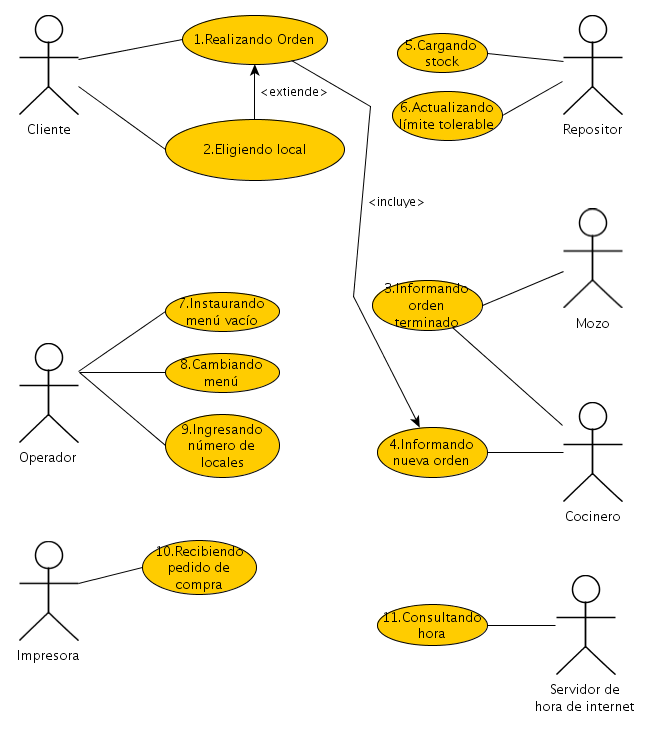
\includegraphics[width=1.3\textwidth]{Imagenes/CasosDeUso.png}}
\caption{Diagrama de Casos de Uso}
\end{figure}


\subsubsection*{Detalles Casos de Uso}
\addcontentsline{toc}{subsubsection}{Detalles de Casos de Uso}

A continuaci\'on se detallar\'a cada caso de uso, dando la descripci\'on de la sucesi\'on de hechos, adem\'as de los actores y la pre y postcondici\'on.

Para seguir un hilo conductor, los casos de uso se encuentran numerados en forma secuencial agrupados por el o los actores participantes.

Se seguir\'a este mismo secuenciamiento para realizar la descripci\'on.

\bigskip


En primer lugar se encuentra unos de los casos de uso m\'as importante en todo el funcionamiento de la pizzer\'ia. La realizaci\'on de un nuevo
pedido por parte del cliente.


\begin{center}
\begin{tabularx}{14cm}{|X|X|}
\hline
\multicolumn{2}{|l|}{Nombre Casos de uso: Realizando orden}\\
\hline
\multicolumn{2}{|l|}{Actores: Cliente}\\
\hline
\multicolumn{2}{|l|}{Precondici\'on: True}\\
\hline
\multicolumn{2}{|l|}{PostCondici\'on: Se logra hacer el pedido}\\
\hline
Curso Normal & Curso Alternativo\\
\hline
1.1 El cliente realiza una orden. & 1.2 La orden no es válida. Fin de C.U.
\\
\hline
2.1 El sistema verifica que se puede realizar la orden (si hay stock). &
\\
\hline
3.1 En caso de que haya stock, el sistema toma el pedido. &
\\
\hline
3.1.1 Se incluye el caso de uso ``Informando nueva orden''. &
\\
\hline
4.1 En caso de que no haya stock, el sistema notifica que no se puede realizar el pedido. &
\\
\hline
4.1.1 Se extiende al caso de uso ``Eligiendo local''. &
\\
\hline
5.1 Fin del C.U. & \\
\hline
\end{tabularx}
\end{center}


\bigskip

\begin{center}
\begin{tabularx}{14cm}{|X|X|}
\hline
\multicolumn{2}{|l|}{Nombre Casos de uso: Eligiendo Local}\\
\hline
\multicolumn{2}{|l|}{Actores: Cliente}\\
\hline
\multicolumn{2}{|l|}{Precondici\'on: El cliente realiz\'o un pedido que no se puede efectuar en el propio local}\\
\hline
\multicolumn{2}{|l|}{PostCondici\'on: El cliente elige un nuevo local}\\
\hline
Curso Normal & Curso Alternativo\\
\hline
1.1 El cliente recibe una lista de locales donde se puede satisfacer su pedido & 
\\
\hline
2.1 El cliente elige un local de la lista recibida & 2.2 El cliente no eligen ning\'ung local. Ir a 4.1.
\\
\hline
3.1 El software debe informar la nueva orden en el local elegido. Se incluye Caso de Uso Informando Nueva Orden &
\\
\hline
4.1 Fin Caso de Uso &
\\
\hline
\end{tabularx}
\end{center}

Este caso de uso, en contraste a la mayor\'ia de los dem\'as, contiene una precondici\'on. Este se incluye para imponer una restricci\'on que no
se puede imponer desde el diagrama mismo dado a que no existe expresividad para esto. 

La precondici\'on del caso de uso dice El cliente realiz\'o un pedido que no se puede efectuar en el propio local.
Esta precondici\'on se incluye para mostrar que este caso de uso no tiene sentido por si solo sin una precedencia directa del caso de uso
Realizando Nueva Orden. Esto no se puede expresar en el diagrama mismo dado que la etiqueta presente en la relaci\'on entre los dos casos de uso 
aparece la etiqueta extiende. Esto es as\'i dado que no siempre que se realiza una nueva orden se elige otro local, por lo que no ser\'ia correcta
la inclusi\'on de una etiqueta incluye. Luego, se usa esta precondici\'on para indicar esta restricci\'on y para poder la descripci\'on del caso de uso
ya asumiendo que el cliente realiz\'o una orden que no pudo ser satisfecha en el propio local.

\bigskip

\begin{center}
\begin{tabularx}{14cm}{|X|X|}
\hline
\multicolumn{2}{|l|}{Nombre Casos de uso: Informando Orden Terminada}\\
\hline
\multicolumn{2}{|l|}{Actores: Mozo, Cocinero}\\
\hline
\multicolumn{2}{|l|}{Precondici\'on: Existe una orden en proceso}\\
\hline
\multicolumn{2}{|l|}{PostCondici\'on: Se informa que hay se finaliz\'o una orden}\\
\hline
Curso Normal & Curso Alternativo\\
\hline
1.1 El cocinero cocina una pizza que se encontraba en una orden en proceso & 
\\
\hline
2.1 El cocinero ingresa en el sistema la finalizaci\'on de la orden pertinente & 
\\
\hline
3.1 El software actualiza el sistema de ordenes, tildando como realizada la orden que el cocinero notific\'o &
\\
\hline
4.1 El software avisa al mozo correspondiente que la orden se encuentra finalizada para retirar &
\\
\hline
5.1 El mozo se entera que se termin\'o una orden y queda dispuesto a ir a buscar la orden para su entrega &
\\
\hline
\end{tabularx}
\end{center}

\bigskip

\begin{center}
\begin{tabularx}{14cm}{|X|X|}
\hline
\multicolumn{2}{|l|}{Nombre Casos de uso: Informando nueva orden}\\
\hline
\multicolumn{2}{|l|}{Actores: Cocinero}\\
\hline
\multicolumn{2}{|l|}{Precondici\'on: Un cliente realizo un pedido}\\
\hline
\multicolumn{2}{|l|}{PostCondici\'on: El cocinero es informado de la nueva orden a realizar}\\
\hline
Curso Normal & Curso Alternativo\\
\hline
1.1 El software, luego de procesar el pedido del cliente, informa al cocinero sobre la nueva orden & 
\\
\hline
2.1 El cocinero es notificado de la nueva orden y se dispone a su realizaci\'on & 
\\
\hline
\end{tabularx}
\end{center}


\medskip

Se puede notar que los casos de uso descriptos hasta el momento se encuentran bastante relacionados, dado que todos juntos conforman una secuencia
com\'un de una cena completa de un cliente en un determinado local. Si bien esta relaci\'on es evidente, en el diagrama de casos de uso no se encuentran
en un hilo secuencial dado que esto no es correcto. Desde un punto de vista de casos de usos at\'omicos no ser\'ia correcto relacionar todos los casos de uso
anteriormente descriptos ya que por ejemplo, entre la realizaci\'on de una nueva orden y la informaci\'on de una orden finalizada pueden pasar horas
en el medio y muchos otros sucesos, por lo que no ser\'ia correcto unirlos en el diagrama.


Sin embargo, como la relaci\'on secuencial es notor\'ia, estos casos de uso ser\'an posteriormente agrupados en un diagrama de actividad que muestre
un hilo de ejecuci\'on completo.

\bigskip

\begin{center}
\begin{tabularx}{14cm}{|X|X|}
\hline
\multicolumn{2}{|l|}{Nombre Casos de uso: Cargando Stock}\\
\hline
\multicolumn{2}{|l|}{Actores: Repositor}\\
\hline
\multicolumn{2}{|l|}{Precondici\'on: True}\\
\hline
\multicolumn{2}{|l|}{PostCondici\'on: Se carga el stock en el sistema}\\
\hline
Curso Normal & Curso Alternativo\\
\hline
1.1 El repositor recibe nuevo stock de alg\'un proveedor & 
\\
\hline
2.1 El repositor ingresa al sistema el stock a actualizar & 
\\
\hline
3.1 El software actualiza el stock de los productos que fueron sumados al deposito de ingredientes &
\\
\hline
4.1 Fin Caso de Uso &
\\
\hline
\end{tabularx}
\end{center}


\bigskip

\begin{center}
\begin{tabularx}{14cm}{|X|X|}
\hline
\multicolumn{2}{|l|}{Nombre Casos de uso: Actualizando l\'imite tolerable}\\
\hline
\multicolumn{2}{|l|}{Actores: Repositor}\\
\hline
\multicolumn{2}{|l|}{Precondici\'on: True}\\
\hline
\multicolumn{2}{|l|}{PostCondici\'on: Se actualiza el l\'imite tolerable de alg\'un producto}\\
\hline
Curso Normal & Curso Alternativo\\
\hline
1.1 El repositor decide modificar el l\'imite tolerable de alg\'un ingrediente en particular & 
\\
\hline
2.1 El repositor ingresa al sistema el ingrediente que quiere actualizar y su correspondiente l\'imite actualizado & 
\\
\hline
3.1 El software actualiza el l\'imite tolerable para el ingrediente que fue se\~{n}alado &
\\
\hline
4.1 Fin Caso de Uso &
\\
\hline
\end{tabularx}
\end{center}


\bigskip
La igual que sucedio con los primeros casos de uso, los casos de uso 5 y 6 tambi\'en se encuentran correlacionados aunque at\'omicamente no lo est\'en.
A su vez, tambi\'en es claro que en una secuencia de acciones del mundo real, estos casos de uso podr\'ian estar relacionados con los casos
de uso 1(realizando orden) y 10(recibiendo pedido de compra). Estas relaciones secuenciales se ver\'an modeladas posteriormente en el diagrama de actividad
referente a todo lo que sucede con respecto al stock cuando se realiza una orden.

\bigskip


\begin{center}
\begin{tabularx}{14cm}{|X|X|}
\hline
\multicolumn{2}{|l|}{Nombre Casos de uso: Instaurando Men\'u vacio}\\
\hline
\multicolumn{2}{|l|}{Actores: Operador}\\
\hline
\multicolumn{2}{|l|}{Precondici\'on: True}\\
\hline
\multicolumn{2}{|l|}{PostCondici\'on: Se carga el men\'u vacio en el sistema}\\
\hline
Curso Normal & Curso Alternativo\\
\hline
1.1 El Operador carga un men\'i vacio al sistema & 
\\
\hline
2.1 El sistema se actualiza para trabajar con este nuevo men\'u vacio & 
\\
\hline
3.1 Fin Caso de Uso &
\\
\hline
\end{tabularx}
\end{center}

\bigskip

\begin{center}
\begin{tabularx}{14cm}{|X|X|}
\hline
\multicolumn{2}{|l|}{Nombre Casos de uso: Cambiando Men\'u}\\
\hline
\multicolumn{2}{|l|}{Actores: Operador}\\
\hline
\multicolumn{2}{|l|}{Precondici\'on: True}\\
\hline
\multicolumn{2}{|l|}{PostCondici\'on: Se actualiza el men\'u}\\
\hline
Curso Normal & Curso Alternativo\\
\hline
1.1 El operador posee una nueva actualizaci\'on para el men\'u & 
\\
\hline
2.1 El operador carga en el sistema la actualizaci\'on & 
\\
\hline
3.1 El software mira el n\'umero de local al que pertenece el operador &
\\
\hline
4.1 El software consulta la hora. Se incluye Casos de uso 11 &
\\
\hline
5.1 El software calcula si el operador se encuentro apto para modificar el men\'u & El operador no se encuentra apt\'o. Ir a 7.1
\\
\hline
6.1 El software actualiza el men\'u &
\\
\hline
7.1 Fin Caso de Uso &
\\
\hline
\end{tabularx}
\end{center}

\bigskip

\begin{center}
\begin{tabularx}{14cm}{|X|X|}
\hline
\multicolumn{2}{|l|}{Nombre Casos de uso: Ingresando n\'umero de locales}\\
\hline
\multicolumn{2}{|l|}{Actores: Operador}\\
\hline
\multicolumn{2}{|l|}{Precondici\'on: True}\\
\hline
\multicolumn{2}{|l|}{PostCondici\'on: Se ingresan los n\'umeros de los locales}\\
\hline
Curso Normal & Curso Alternativo\\
\hline
1.1 El Operador carga los n\'umeros asignados a cada local & 
\\
\hline
2.1 El sistema actualiza los n\'umeros de los locales para realizar los c\'alculos de round robin & 
\\
\hline
3.1 Fin Caso de Uso &
\\
\hline
\end{tabularx}
\end{center}

\bigskip

Los 3 casos de uso anteriormente descriptos son los que m\'as estan relacionados con el hecho de la actualizaci\'on del men\'u. Esto, como ya se
explic\'o con anterioridad, se mostrar\'a de una manera m\'as visual en un diagrama de actividad que muestre lo que sucede al actualizar un men\'u
en el mundo y en la interfaz. Mientras que luego, con una m\'aquina de estados, se modelar\'a lo que sucede dentro de la m\'aquina con esta acci\'on.

\bigskip

\begin{center}
\begin{tabularx}{14cm}{|X|X|}
\hline
\multicolumn{2}{|l|}{Nombre Casos de uso: Recibiendo pedido de compra}\\
\hline
\multicolumn{2}{|l|}{Actores: Impresora}\\
\hline
\multicolumn{2}{|l|}{Precondici\'on: True}\\
\hline
\multicolumn{2}{|l|}{PostCondici\'on: La impresora recibe un nuevo pedido de compra}\\
\hline
Curso Normal & Curso Alternativo\\
\hline
1.1 El software posee uno o muchos ingrendientes que deben ser repuestos & 
\\
\hline
2.1 El software genera el pedido de compra para satisfacer la necesidades calculadas & 
\\
\hline
3.1 El software manda a la impresora la correspondiente orden de compra &
\\
\hline
4.1 Fin Caso de Uso &
\\
\hline
\end{tabularx}
\end{center}

\bigskip

\begin{center}
\begin{tabularx}{14cm}{|X|X|}
\hline
\multicolumn{2}{|l|}{Nombre Casos de uso: Consultando Hora}\\
\hline
\multicolumn{2}{|l|}{Actores: Servidor de hora de internet}\\
\hline
\multicolumn{2}{|l|}{Precondici\'on: Un operador esta intentando actualizar el men\'u}\\
\hline
\multicolumn{2}{|l|}{PostCondici\'on: Se obtiene una actualizaci\'on de la hora}\\
\hline
Curso Normal & Curso Alternativo\\
\hline
1.1 El software requiere la hora para calculos de round robin & 
\\
\hline
2.1 El Software le pide al servidor una actualizaci\'on de la hora & 
\\
\hline
3.1 El Servidor devuelve lo solicitado al software &
\\
\hline
4.1 Fin Caso de Uso &
\\
\hline
\end{tabularx}
\end{center}

\newpage

\subsection*{Diagramas de Actividad}
\addcontentsline{toc}{subsection}{Diagrmas de Actividad}


Los diagramas de actividad son una representaci\'on para mostrar el secuenciamiento de varias acciones que se encuentran relacionadas por alg\'un
hilo conductor. Los diagramas de actividad se encuentran enriquecedos por el hecho de poder soportar varios actores en un mismo hilo mediante la 
separaci\'on por andariveles de las interacciones de cada actor, es por esto que son muy adecuados para modelar las acciones que suceden entre la
m\'aquina y los actores externos e incluso las acciones que suceden entre los actores externos sin interacci\'on con la m\'aquina.

Si bien las interacciones entre el mundo y la m\'aquina ya fueron descriptas en el diagrama de casos de uso, se realiz\'o de forma diferente
ya que la t\'ecnica de casos de uso se basa en centrarse at\'omicamente en cada caso de uso y solo se explicita una relaci\'on entre dos casos de
uso cuando la relaci\'on es inmediata.

En contraposici\'on a los casos de uso, se utilizar\'an los diagramas de actividad para modelar las secuencias de acciones que sucederi\'an en la 
pizzer\'ia, sin centrarse en cada paso de la secuencia particularmente (dado que ya fueron explayados en los casos de uso).

Se decidi\'o que la t\'ecnica ser\'ia utlizada para los siguientes casos particulares:

\begin{itemize}
\item El ciclo de vida completo de una orden.
\item Ejemplo de manejo de stock.
\item Actualizaci\'on del men\'u.
\end{itemize}


\subsubsection*{Ciclo de vida de una orden}
\addcontentsline{toc}{subsubsection}{Ciclo de vida de una orden}

Este diagrama de actividad sirve para agrupar las acciones sucecidas en el ciclo de vida de una orden, es decir desde el momento que un cliente
pide una orden hasta el momento que recibe su pizza(o bien no la recibe porque no se puede satisfacer). Cabe destacar que en el diagrama de actividad
se abstraen varias situaciones para centrarse solamente en la orden en s\'i. Es decir, si bien usar los ingrendientes para realizar una orden podr\'ia
desencadenar un pedido al proveedor, no ser\'a modelado en este diagrama, sino en el siguiente.

En este diagrama se destaca la diferencia entre que el pedido se cocine en el local donde el cliente se encuentra o en otro, por lo que se 
diferencian entre el cocinero y el mozo del local propio y el cocinero y el mozo del local externo donde el cliente va a ir a buscar la pizza.

% aca va el diagrama de actividad de ciclo de vida de una orden

\bigskip

\subsubsection*{Ejemplo de manejo de stock}
\addcontentsline{toc}{subsubsection}{Ejemplo de manejo de stock}

Este diagrama de actividad se utilizar\'a para modelar las acciones pertinentes al manejo de stock cuando se realiza una orden. Dado que solo
se quiere modelar lo relacionado con el stock, ya que los otros aspectos respectivos a la realizaci\'on de una orden fueron modelados anteriormente,
el diagrama presenta una secuencia de acciones donde un cliente realiza una orden que se puede satisfacer por dicho local para poder mostrar concretamente
que sucede con el stock sin p\'erdida de generalidad.

% aca va el diagrama de actividad de manejo de stock

\bigskip

\subsubsection*{Actualizaci\'on del men\'u}
\addcontentsline{toc}{subsubsection}{Actualizaci\'on del men\'u}

Este diagrama de actividad sirve para modelar el hilo de ejecuci\'on de las acciones referidas a la actualizaci\'on de un men\'u en cuanto a la interacci\'on
de los actores externos participantes con la m\'aquina. Lo que sucede dentro de la m\'aquina para mantener una consistencia entre los locales es inherente
a la m\'aquina misma por lo que ser\'a modelado posteriormente con la t\'ecnica de m\'aquinas de estados.

% aca va el diagrama de actividad de actualizacion de menu


\bigskip

\subsection*{M\'aquinas de Estado Finita}
\addcontentsline{toc}{subsection}{M\'aquinas de Estado Finita}


\newpage


\section*{Discusi\'on}
\addcontentsline{toc}{section}{Discusi\'on}




\newpage
\section*{Conclusiones}
\addcontentsline{toc}{section}{Conclusiones}





\end{document}
